%        File: arfc-beamer.tex
%     Created: Sun May 5 10:00 PM 2013 C
%


%\documentclass[11pt,handout]{beamer}
\documentclass[9pt]{beamer}
\usetheme[white]{Illinois}
\title[Short Title]{Fluoride-Salt-Cooled High-Temperature Reactor Design Optimization with Evolutionary Algorithms \\ Preliminary Exam}
\author[Your Name]{Gwendolyn J.Y. Chee}
\date[09.13.2021]{September 13, 2021}
\institute{
Dept. of Nuclear, Plasma and Radiological Engineering \\ University of Illinois at Urbana-Champaign
}

%\usepackage{bbding}
\usepackage{amsfonts}
\usepackage{amsmath}
\usepackage{xspace}
\usepackage{graphicx}
\usepackage{booktabs} % nice rules for tables
\usepackage{microtype} % if using PDF
\usepackage{bigints}
\usepackage{minted}

\newcommand{\Cyclus}{\textsc{Cyclus}\xspace}%
\newcommand{\Cycamore}{\textsc{Cycamore}\xspace}%
\newcommand{\deploy}{\texttt{d3ploy}\xspace}%
\newcommand{\units}[1] {\:\text{#1}}%
\newcommand{\SN}{S$_N$}%{S$_\text{N}$}%{$S_N$}%
\DeclareMathOperator{\erf}{erf}
%I need some complimentary error funcitons... 
\DeclareMathOperator{\erfc}{erfc}
%page numbers
\setbeamertemplate{footline}[page number]
\setbeamertemplate{caption}[numbered]
%Those icons in the references are terrible looking
\setbeamertemplate{bibliography item}[text]

\usepackage{tkz-euclide}
\usepackage{tikz}
\usetikzlibrary{positioning, arrows, decorations, shapes}

\usetikzlibrary{shapes.geometric,arrows}
\tikzstyle{process} = [rectangle, rounded corners, minimum width=3cm, minimum height=1cm,text centered, draw=black, fill=blue!30]
\tikzstyle{object} = [ellipse, rounded corners, minimum width=3cm, minimum height=1cm,text centered, draw=black, fill=green!30]
\tikzstyle{arrow} = [thick,->,>=stealth]

\definecolor{illiniblue}{HTML}{B1C6E2}
\definecolor{illiniorange}{HTML}{f8c2a2}
\definecolor{illinigreen}{HTML}{a0deb1}
\definecolor{grey}{HTML}{dce3de}
\usetikzlibrary{shapes.geometric, arrows}
\tikzstyle{oblock} = [rectangle, draw, fill=illiniorange, 
text width=9em, text centered, rounded corners, minimum height=4em]
\tikzstyle{bblock} = [rectangle, draw, fill=illiniblue, 
text width=8em, text centered, rounded corners, minimum height=4em]
\tikzstyle{gblock} = [rectangle, draw, fill=illinigreen, 
text width=8em, text centered, rounded corners, minimum height=4em]
\tikzstyle{lgblock} = [rectangle, draw, fill=illinigreen, 
text width=9em, text centered, rounded corners, minimum height=4em]
\tikzstyle{noblock} = [rectangle,
text width=8em, text centered, minimum height=4em]
\tikzstyle{greyblock} = [rectangle, fill=grey, 
text width=8em, minimum height=4em, rounded corners]
\tikzstyle{lgreyblock} = [rectangle, fill=grey, 
text width=9em, minimum height=4em, rounded corners]
\tikzstyle{llgreyblock} = [rectangle, fill=grey, 
text width=20em, minimum height=4em, rounded corners]
\tikzstyle{arrow} = [thick,->,>=stealth]

\definecolor{fhrblue}{HTML}{0000ff}
\definecolor{fhrgrey}{HTML}{808080}
\definecolor{fhrred}{HTML}{f10a0a}
\definecolor{fhrgreen}{HTML}{2f6d39}
\definecolor{fhryellow}{HTML}{fdfe36}

\usepackage{tabularx}
\newcolumntype{b}{>{\hsize=1.0\hsize}X}
\newcolumntype{s}{>{\hsize=.5\hsize}X}
\newcolumntype{m}{>{\hsize=.75\hsize}X}
\newcolumntype{x}{>{\hsize=.25\hsize}X}
\newcolumntype{L}{>{\raggedright\arraybackslash}X}
\newcolumntype{R}{>{\raggedleft\arraybackslash}X}
\def\arraystretch{1}
%%%% Acronym support
\usepackage{multirow}
\usepackage{graphicx}
\usepackage{subcaption}

\usepackage[acronym,toc]{glossaries}
\include{acros}

\makeglossaries
\setbeamerfont{subsection in toc}{size=\scriptsize}

%try to get rid of header on title page\dots
\makeatletter
    \newenvironment{withoutheadline}{
        \setbeamertemplate{headline}[default]
        \def\beamer@entrycode{\vspace*{-\headheight}}
    }{}
\makeatother

% add slide numbers
\makeatother
\setbeamertemplate{footline}
{
  \leavevmode%
  \hbox{%
    \rightline{\insertframenumber{} / \inserttotalframenumber\hspace*{1ex}}
  }%
  \vskip0pt%
}
\makeatletter

\begin{document}
%%%%%%%%%%%%%%%%%%%%%%%%%%%%%%%%%%%%%%%%%%%%%%%%%%%%%%%%%%%%%
%% From uw-beamer Here's a handy bit of code to place at 
%% the beginning of your presentation (after \begin{document}):
\newcommand*{\alphabet}{ABCDEFGHIJKLMNOPQRSTUVWXYZabcdefghijklmnopqrstuvwxyz}
\newlength{\highlightheight}
\newlength{\highlightdepth}
\newlength{\highlightmargin}
\setlength{\highlightmargin}{2pt}
\settoheight{\highlightheight}{\alphabet}
\settodepth{\highlightdepth}{\alphabet}
\addtolength{\highlightheight}{\highlightmargin}
\addtolength{\highlightdepth}{\highlightmargin}
\addtolength{\highlightheight}{\highlightdepth}
\newcommand*{\Highlight}{\rlap{\textcolor{HighlightBackground}{\rule[-\highlightdepth]{\linewidth}{\highlightheight}}}}
%%%%%%%%%%%%%%%%%%%%%%%%%%%%%%%%%%%%%%%%%%%%%%%%%%%%%%%%%%%%%
%%--------------------------------%%
\begin{withoutheadline}
\frame{
  \titlepage
}
\end{withoutheadline}

%%--------------------------------%%
\AtBeginSection[]{
\begin{frame}
  \frametitle{Outline}
  \tableofcontents[currentsection]
\end{frame}
}

\section{Introduction}
\subsection{Motivation: AHTR Model Development}
\begin{frame}
    \frametitle{Why Generation IV Reactors?}
    \begin{itemize}
      \item Energy use and production contribute two-thirds of total \gls{GHG} emissions \cite{noauthor_climate_2018}
      \item Because energy generation technology selection profoundly impacts climate change, 
      large scale emissions-free nuclear power deployment could 
      significantly reduce GHG production but faces both cost and perceived adverse 
      safety challenges \cite{noauthor_climate_2018, petti_future_2018}.
      \item The Generation IV International Forum identified six Generation IV systems 
      that target goals in four areas: sustainability, 
      economics, safety and reliability, and proliferation resistance and physical 
      protection: GFR, LFR, MSR, SFR, SCWR, and VHTR. 
      \begin{figure}[htbp!]
          \includegraphics[height=2.8cm]{figures/msr}
          \hspace{1cm}
          \includegraphics[height=2.8cm]{figures/vhtr}
      \end{figure}
    \end{itemize}
  \end{frame}
\begin{frame}
  \frametitle{MSRs and VHTRs}
  \begin{block}{Molten Salt Reactor (MSR) System}
    \begin{itemize}
      \item Produces fission power in circulating molten salt fuel mixture
      \item Molten Fluoride Salts have have chemical stability, low vapor pressure 
      at high temperatures, good heat transfer properties, resistance against 
      radiation damage, and inert to common structural materials
      \item Inherent system safety with fail-safe drainage, passive cooling, and 
      low inventory of volatile fission products in the fuel
    \end{itemize}
  \end{block}
  \vspace{-0.25cm}
  \begin{block}{Very High Temperature Reactor System (VHTR)}
    \begin{itemize}
      \item Tristructural Isotropic (TRISO) fuel withstands high burnup and 
      temperature
      \item High outlet temperature increases power conversion efficiency, reduces 
      waste heat generation, and enables high-temperature heat applications 
      such as hydrogen production
      \item Helium coolant's high 100 atm pressurization requires an expensive thick
      concrete reactor vessel
    \end{itemize}
  \end{block}
\end{frame}
\begin{frame}
  \frametitle{FHR}
  \begin{itemize}
    \item \acrlong{FHR} concept combines the best aspects of \acrlong{MSR} and \acrlong{VHTR} technologies. 
      \acrshort{FHR} use high-temperature coated-particle fuel (similar to the \acrshortpl{VHTR}) 
      and a low-pressure liquid fluoride-salt coolant (similar to the \acrshortpl{MSR})
      \cite{forsberg_fluoride-salt-cooled_2012,facilitators_fluoride-salt-cooled_2013}.
  \end{itemize}
  \begin{block}{\acrfull{FHR} Benefits}
    \begin{itemize}
      \item FHR system has low operating pressure, thus does not require thick 
      concrete pressure vessel 
      \item Molten salt coolant has superior cooling and moderating properties 
      compared to helium coolant in VHTRs
      \item FHR system has large thermal margin enabled by molten salt coolant
      \item FHRs' TRISO particles' solid fuel cladding adds an extra barrier to 
      fission product release compared to MSRs with liquid fuel.
    \end{itemize}
  \end{block}
\end{frame}
\begin{frame}
  \frametitle{AHTR}
  \begin{block}{Advanced High Temperature Reactor Design}
    \begin{itemize}
      \item Design developed by Oak Ridge National Laboratory (ORNL)
      \item Prismatic FHR design with 252 hexagonal fuel assemblies consisting of 
      18 fuel planks arranged in 3 diamond-shaped sectors. 
    \end{itemize}
  \end{block}
  \begin{figure}[]
    \centering
    \includegraphics[width=0.8\linewidth]{../docs/figures/ahtr.png} 
    \caption{\acrlong{AHTR} fuel assembly (left) and core configuration (right) 
    reproduced from \cite{ramey_monte_2018}.}
    \label{fig:ahtr}
\end{figure}
\end{frame}

\begin{frame}
  \frametitle{AHTR Geometry}
  \begin{block}{Advanced High Temperature Reactor Design}
    \begin{itemize}
      \item Each fuel plank contains 2 fuel stripes that consists of a cubic 
      lattice of TRISO fuel particles
    \end{itemize}
  \end{block}
  \vspace{-0.3cm}
  \begin{figure}[]
    \includegraphics[width=0.45\linewidth]{figures/ahtr-assembly.png} 
    \includegraphics[width=0.45\linewidth]{figures/ahtr-plank.png} 
    \caption{\acrfull{AHTR} fuel assembly with 18 fuel plates arranged in 
    three diamond-shaped sectors, with a central Y-shaped and external channel 
    graphite structure.}
\end{figure}
\end{frame}

\begin{frame}
  \frametitle{FHR Benchmark}
  \begin{itemize}
    \item The AHTR's fuel geometry has triple heterogeneity resulting in
    complex reactor physics and significant modeling challenges
    \item To address and further understand the technical challenges for 
    AHTR modeling, in 2019 the OECD-NEA initiated a FHR benchmark exercise. Its objective 
    is to identify the applicability, accuracy, and practicality of the latest 
    methods and codes to assess the current state of the art of FHR simulation 
    and modeling. The benchmark also enables the cross-verification of software 
    and methods for the challenging AHTR geometry, which is especially useful 
    since applicable reactor physics experiments for code validation are scarce
  \end{itemize}
  \begin{figure}[]
    \includegraphics[width=0.5\linewidth]{figures/benchmark.png} 
    \caption{OECD NEA's FHR Benchmark \cite{petrovic_benchmark_2021}.}
\end{figure}
\end{frame}


\subsection{Objectives: AHTR Model Development}
\begin{frame}
  \frametitle{Research Objectives}
  \begin{block}{Technical Gap}
    \begin{itemize}
      \item The triple heterogeneity introduced by the geometrically complex 
      fuel assembly design makes accurate reactor physics simulations challenging. 
      Thus requiring a need to access accuracy of such analyses 
    \end{itemize}
  \end{block}
  \begin{block}{Proposed Work Component I: AHTR Model Development}
    \begin{itemize}
      \item I aim to further our understanding of the AHTR design's complexities 
      through neutronics and thermal-hydraulics modeling.
      \item I will participate in the OECD-NEA's FHR Benchmarking exercise with 
      OpenMC and Moltres
      \item Objectives 
      \begin{itemize}
        \item AHTR 2D and 3D assembly neutronics steady state and depletion models 
        with neutron transport software, OpenMC
        \item AHTR 2D fuel plank and assembly neutronics with thermal hydraulics 
        feedback using Moltres
      \end{itemize}
    \end{itemize}
  \end{block}
\end{frame}

\subsection{Motivation: AHTR Optimization}
\begin{frame}
    \frametitle{Motivation}
    \begin{block}{Impact of Additive Manufacturing Technology Advancements on 
        Reactor Design Optimization}
        \begin{itemize}
            \item Additive manufacturing technology, popularly known as `3D printing', 
            has advanced and altered the manufacturing and design of engineered hardware
            \cite{simpson_considerations_2019}. 
            \item With further advancement of additive manufacturing technologies, a reactor 
            core could be 3D printed in the near future. 
            \acrlong{ORNL} leads this initiative through the 2019 \acrlong{TCR} Demonstration 
            Program. 
            \item Leveraging additive manufacturing technology enables us to surpass classical 
            manufacturing constraints, such as straight fuel channels or homogenous fuel 
            enrichment, and optimize for arbitrary geometries and parameters 
            such as non-uniform channel shapes, and inhomogeneous fuel distribution 
            throughout the core. 
          \end{itemize}
    \end{block}
  \end{frame}

  \begin{frame}
    \frametitle{Motivation}
    \begin{block}{Evolutionary Algorithms for Reactor Design Optimization}
        \begin{itemize}
            \item Evolutionary algorithms have proven successful in optimizing multi-objective 
            problems such as reactor design optimization, as they can find solutions at the global 
            optimum and also take advantage of parallel systems. 
            \item Evolutionary algorithms imitate natural selection to evolve solutions 
            \cite{renner_genetic_2003}:
            \begin{itemize}
                \item maintaining a population of solutions
                \item allowing more optimal solutions to reproduce 
                \item letting less optimal solutions to die off resulting in 
                solutions that are better than previous generations
            \end{itemize}
            \end{itemize}
    \end{block}
  \end{frame}
    

\subsection{Objectives: AHTR Optimization}
\begin{frame}
    \frametitle{Research Objectives}
    \begin{block}{Technical Gap}
      \begin{itemize}
        \item Previous efforts towards nuclear reactor optimization focuses
        on optimizing classical reactor parameters such as radius of fuel pellet 
        and clad, enrichment of fuel, pin pitch, etc.
        \item Additive manufacturing advancements enable reactor designers to 
        optimize beyond conventional manufacturing shapes that are easy to 
        manufacture such as slabs as fuel planks, cylinders as rods, axis-aligned
        coolant channels 
        \item Applying evolutionary algorithms to nuclear design problems is not new,
        however, evolutionary algorithm setup is highly customizable, A reactor 
        designer unfamiliar with evolutionary algorithms will have to go through 
        the cumbersome process of customizing a genetic algorithm for their
        needs and determine which operators and hyperparameters work best for their problem
      \end{itemize}
    \end{block}
    \begin{block}{Scope 2: }
      \begin{itemize}
        \item f
        \end{itemize}
    \end{block}
  \end{frame}

\section{Methodology}
\subsection{FHR Benchmark Specifications}
\begin{frame}
    \frametitle{FHR Benchmark Specifications}
    \begin{itemize}
        \item Several organizations participate in the benchmark with various Monte Carlo
        and Deterministic neutronics software, such as Serpent \cite{leppanen_serpent_2014}, 
        OpenMC \cite{romano_openmc_2013}, and WIMS \cite{lindley_current_2017}. 
        \item UIUC participates in the benchmark with the OpenMC Monte Carlo code 
        \cite{romano_openmc_2013} using the ENDF/B-VII.1 material cross section library 
        \cite{chadwick_endf/b-vii.1_2011}.
        \item The benchmark will have three phases, starting from a single fuel assembly
        simulation without burnup (Phase I), gradually extending to full core depletion
        (Phase II) and multi-physics feedback (Phase III). 
    \end{itemize}
    \vspace{-0.2cm}
    \begin{table}
        \caption{OECD NEA's FHR Benchmark Phases 
        \cite{petrovic_benchmark_2021}.}
        \vspace{-0.25cm}
        \includegraphics[width=0.9\linewidth]{figures/benchmark-phases.png} 
    \end{table}
\end{frame}

\begin{frame}
    \frametitle{FHR Benchmark Specifications}
    \begin{itemize}
        \item Only Phase I-A and I-B specifications have been released 
        \item Benchmark participants must produce the following results for 
        the 9 cases: $k_{eff}$, reactivity coefficients ($\beta_{eff}$, 
        $\alpha_D$, $\alpha_{T, FliBe}$, $\alpha_M$), fission source distribution, 
        neutron flux distribution, fuel assembly averaged neutron spectrum
    \end{itemize}
    \vspace{-0.25cm}
    \begin{table}
        \caption{Description of the \acrlong{FHR} benchmark Phase I-A cases 
        \vspace{-0.25cm}
        \cite{noauthor_fluoride_nodate}.}
        \includegraphics[width=0.8\linewidth]{figures/benchmark-cases.png} 
    \end{table}
\end{frame}
\subsection{ROLLO Tool Design}
\begin{frame}
    \frametitle{Proposed Tool's Design Goals}
    \begin{itemize}
        \item ROLLO (Reactor evOLutionary aLgorithm Optimizer) is a Python package 
        that applies evolutionary algorithm techniques to optimize nuclear reactor design.
        \item ROLLO couples an evolutionary algorithm driver, Distributed 
        Evolutionary Algorithms in Python (DEAP), with 
        nuclear software, such as neutron transport OpenMC and thermal-hydraulics 
        Moltres codes.
    \end{itemize}
    \begin{block}{ROLLO Design Goals}
        \begin{itemize}
            \item Effective: good documentation, well tested, version controlled 
            on Github 
            \item Flexible: user can vary any imaginable parameter because
            ROLLO uses a templating method to edit the input file of the coupled software.
            \item Open-source: utilizes only open-source dependencies 
            \item Parallel: toggle to enable parallelization on local and HPCs
            \item Reproducible: Data from every ROLLO run saves into a unique, 
            pickled file (pickle is a Python module that serializes Python 
            objects), and all results from this work are available on Github.
        \end{itemize}
    \end{block}
\end{frame}

\begin{frame}
    \frametitle{ROLLO Flow Chart}
    \begin{figure}
        \begin{minipage}[c]{0.3\textwidth}
        \caption{Process of finding optimal solutions for a problem with a 
        genetic algorithm. Nuclear software evaluates each new population.}
        \end{minipage}\hfill
        \begin{minipage}[c]{0.7\textwidth}
        \includegraphics[width=\linewidth]{figures/rollo-flow.png} 
        \end{minipage}
    \end{figure}
\end{frame}

\section{Proposed work and preliminary results}
\subsection{Progress Chart}
\begin{frame}
    \frametitle{Proposed Work's Component 1 Progress}
    AHTR Model Development for the FHR Benchmark

    \begin{figure}[]
        \centering
        \resizebox{\textwidth}{!}{
        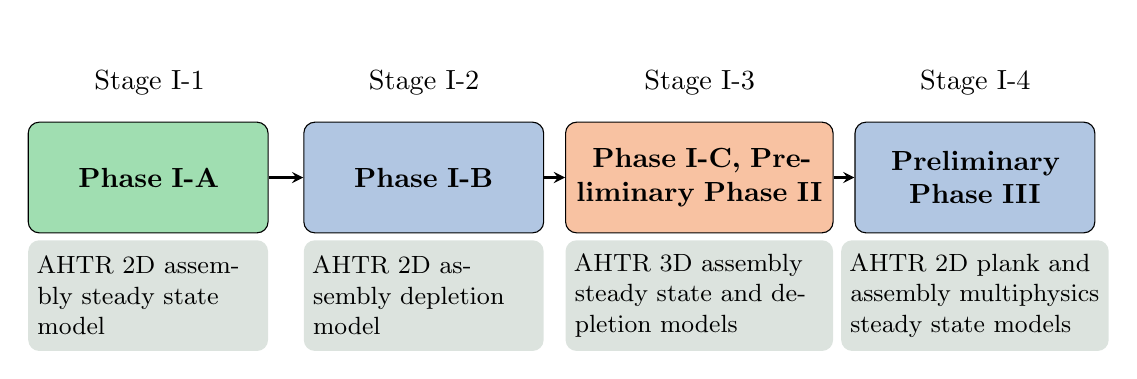
\begin{tikzpicture}[node distance=3.5cm,auto,>=latex']
            \node [gblock] (a) {\textbf{Phase I-A}};
            \node [bblock] (b) [right of=a] {\textbf{Phase I-B}};
            \node [oblock] (c) [right of=b] {\textbf{Phase I-C, Preliminary Phase II}};
            \node [bblock] (d) [right of=c] {\textbf{Preliminary Phase III}};
            \node [noblock] (e) [above of=a, yshift=-2.3cm] {Stage I-1};
            \node [noblock] (e) [above of=b, yshift=-2.3cm] {Stage I-2};
            \node [noblock] (e) [above of=c, yshift=-2.3cm] {Stage I-3};
            \node [noblock] (e) [above of=d, yshift=-2.3cm] {Stage I-4};
            \node [greyblock] (e) [below of=a, yshift= 2cm, font=\small] {AHTR 2D assembly steady state model};
            \node [greyblock] (e) [below of=b, yshift= 2cm, font=\small] {AHTR 2D assembly depletion model};
            \node [lgreyblock] (e) [below of=c, yshift= 2cm, font=\small] {AHTR 3D assembly steady state and depletion models};
            \node [lgreyblock] (e) [below of=d, yshift= 2cm, font=\small] {AHTR 2D plank and assembly multiphysics steady state models};
            \draw [arrow] (a) -- (b);
            \draw [arrow] (b) -- (c);
            \draw [arrow] (c) -- (d);
        \end{tikzpicture}}
    \end{figure}
    \begin{figure}
        \resizebox{0.25\textwidth}{!}{
            \fbox{\begin{tabular}{ll}
                \textcolor{illinigreen}{$\blacksquare$} & Completed \\
                \textcolor{illiniblue}{$\blacksquare$} & In Progress \\
                \textcolor{illiniorange}{$\blacksquare$} & Planned \\
                \end{tabular}}}
    \end{figure}
\end{frame}
\subsection{Stage I-1: FHR Benchmark Phase I-A (Completed)}
\begin{frame}
    \frametitle{Completed Stage I-1: FHR Benchmark Phase I-A Results}
    \begin{itemize}
        \item FHR Benchmark Phase I-A: 2D assembly steady state model
        \item In a recently submitted ANS M$\&$C 2021 conference paper 
        (which I am a co-author on), 
        Petrovic et al. \cite{petrovic_preliminary_2021} compared FHR benchmark 
        participants' Phase I-A $k_{eff}$ results.  
        We reported that the standard deviation between participants for each case 
        was in the 231 to 514 pcm range, acceptable and notably close given a blind 
        benchmark, assuring that \gls{UIUC}'s Phase I-A results are acceptable and 
        in agreement with other benchmark participants 
    \end{itemize}
    \begin{figure}[]
        \begin{minipage}[c]{0.5\textwidth}
        \centering
        \includegraphics[width=0.75\linewidth]{figures/ahtr-assembly.png} 
        \end{minipage}\hfill
        \begin{minipage}[c]{0.5\textwidth}
        \caption{\acrfull{AHTR} fuel assembly with 18 fuel plates arranged in 
        three diamond-shaped sectors, with a central Y-shaped and external channel 
        graphite structure.}
        \end{minipage}
    \end{figure}
\end{frame}

\begin{frame}
    \frametitle{Completed Stage I-1: FHR Benchmark Phase I-A Results}
    \begin{table}
        \caption{\acrlong{UIUC}'s \acrlong{FHR} Benchmark Phase I-A results 
        \cite{chee_arfcfhr-benchmark_2021}.}
        \includegraphics[width=\linewidth]{figures/benchmark-coeff-results.png} 
    \end{table}
\end{frame}

\begin{frame}
    \frametitle{Completed Stage I-1: FHR Benchmark Phase I-A Results}
    \begin{figure}[]
        \centering
        \includegraphics[width=0.6\linewidth]{figures/phase1a-e.png} 
        \caption{UIUC results: FHR Benchmark neutron flux 
        distribution in 100 $\times$ 100 mesh for three coarse energy groups: Case 
        1A (above), Case 3A (middle), Case 6A (below). Energy group 1: $E > 0.1$ MeV, 
        Energy group 2: $3 \times 10^{-6} < E < 0.1$ MeV, Energy group 3: $E < 3 \times 10^{-6}$ MeV. }
    \end{figure}
\end{frame}
\subsection{Stage I-2: FHR Benchmark Phase I-B (In Progress)}
\begin{frame}
    \frametitle{Stage I-2: FHR Benchmark Phase I-B Results}
    \begin{itemize}
        \item FHR Benchmark Phase I-B: 2D assembly depletion model
        \item Benchmark participants are working on resolving differences in 
        these results
    \end{itemize}
    \begin{figure}[]
        \centering
        \includegraphics[width=0.75\linewidth]{../docs/figures/phase1b_keff.png} 
        \caption{UIUC results: FHR Benchmark Phase I-B depletion 
        $k_{eff}$ evolution for Cases 1B, 4B, and 7B. Case 1B is the reference case, 
        Case 4B is the discrete \acrlong{BP} case, and Case 7B is the 19.75$\%$ 
        enrichment case. Error bars are included but are barely visible due to the 
        low $\sim$40pcm uncertainty.}
    \end{figure}
\end{frame}
\subsection{Stage I-3: FHR Benchmark Phase I-C and II (Planned)}
\begin{frame}
    \frametitle{Planned Stage I-3: FHR Benchmark Phase I-C and II Goals}
    \begin{block}{Phase I-C}
        \begin{itemize}
            \item The FHR benchmark's Phase I-C extends the 2D assembly model from 
            Phases I-A and I-B into a 3D assembly model. The benchmark organizers 
            will release the Phase I-C detailed specifications and required results 
            in late 2021.
            \item When the specifications are released, I will contribute Phase I-C
            results to the benchmark. 
        \end{itemize}
    \end{block}
    \begin{block}{Preliminary Phase II}
        \begin{itemize}
            \item FHR Benchmark Phase II: 3D full core steady state and depletion 
            models 
            \item For preliminary work towards Phase II, I will expand the AHTR model 
            from assembly to full core 
        \end{itemize}
    \end{block}
\end{frame}
\subsection{Stage I-4: FHR Benchmark III (Planned)}
\begin{frame}
    \frametitle{In Progress Stage 1-4: FHR Benchmark Phase III Goals}
    \begin{itemize}
        \item FHR Benchmark Phase III: 3D full core with feedback and multicycle 
        analysis
        \item I will use the open-source MSR simulation tool, Moltres, to conduct
        AHTR multiphysics simulations for fuel slab and $\frac{1}{3}$
        fuel assembly geometries 
        \item AHTR Moltres simulations will capture thermal feedback effects, 
        absent from the purely neutronics OpenMC simulations
    \end{itemize}
\end{frame}

\begin{frame}
    \frametitle{In Progress Stage 1-4: Benchmark Phase III Preliminary Work}
    For successful AHTR Moltres simulation, I must establish 
    suitable spatial and energy homogenization that preserves accuracy while 
    maintaining an acceptable runtime
\begin{block}{Spatial Homogenization}
    Fuel slab discretization into 13 cells: FLiBe, left graphite, right graphite, 
    and ten fuel cells (each cell has a different packing fraction)
\end{block}
\begin{figure}[]
    \includegraphics[width=0.8\linewidth]{figures/straightened_slab_mg.png}
    \caption{Straightened AHTR fuel slab spatially discretized into 
    13 \textit{cells} for OpenMC multigroup calculation.}
\end{figure}
\end{frame}

\begin{frame}
    \frametitle{In Progress Stage 1-4: Benchmark Phase III Preliminary Work}
    \begin{block}{Energy Homogenization}
        \begin{table}[]
            \centering
            \begin{minipage}[c]{0.6\textwidth}
                \centering
                \includegraphics[width=0.7\linewidth]{figures/ahtr-energy-discr.png}
            \end{minipage}\hfill
            \begin{minipage}[c]{0.4\textwidth}
            \caption{4-group energy structures for AHTR geometry 
            derived by \cite{gentry_development_2016}.}
        \end{minipage}
        \end{table}
    \end{block}
    \vspace{-0.3cm}
    \begin{block}{Simulation Comparison: Continuous energy vs spatial 
        and energy homogenized}
        \begin{table}[]
                \centering
                \caption{
                    AHTR fuel slab's $k_{eff}$ for case with continuous energy and 
                    space and case with spatial and energy homogenization.}
                \includegraphics[width=0.9\linewidth]{figures/ahtr-homogenization.png}
        \end{table}
    \vspace{-0.3cm}
    Therefore, these homogenizations are suitable for generating group constants 
    for a Moltres simulation. 
    \end{block}
\end{frame}

\begin{frame}
    \frametitle{In Progress Stage 1-4: Benchmark Phase III Planned Work}
    \begin{itemize}
        \item Use these spatial and energy homogenization to set up a 
        Moltres AHTR plank steady-state simulation 
        \item Verify the Moltres model's neutronics parameters then run 
        the steady state simulation to determine maximum temperature 
        \item Test out energy and spatial homogenization methods for $\frac{1}{3}$
        fuel assembly Moltres model 
    \end{itemize}
\end{frame}
\subsection{Stage II-1: ROLLO v1.0 Build}
\begin{frame}
    \frametitle{Completed Stage II-1: ROLLO v1.0 Build}
    \begin{itemize}
        \item ROLLO initially reads and validates the JSON input file, initializes 
        the Distributed Evolutionary Algorithms in Python (DEAP) [25] genetic algorithm 
        hyperparameters and operators, and finally runs the genetic algorithm
    \end{itemize}
    \begin{figure}
        \begin{minipage}[c]{0.7\textwidth}
            \centering
        \includegraphics[width=0.7\linewidth]{figures/rollo-json-input.png} 
        \end{minipage}\hfill
        \begin{minipage}[c]{0.3\textwidth}
        \caption{ROLLO sample JSON input file.}
        \end{minipage}
    \end{figure}
\end{frame}

%\input{acks}
%%--------------------------------%%
%%--------------------------------%%
\begin{frame}[allowframebreaks]
  \frametitle{References}
  \bibliographystyle{plain}
  {\footnotesize \bibliography{../docs/2021-chee-prelim.bib} }

\end{frame}

%%--------------------------------%%


\end{document}



